% Standalone source for the participant selection flow diagram (@fig-prisma).
%
% Wiley/HBM require figures as separate graphics files rather than inline LaTeX,
% so this diagram is compiled to fig-prisma.pdf and included by manuscript.qmd
% via \includegraphics. Edit this file, not the manuscript, to change the figure.
%
% Build:
%   cd reports-src/figures && xelatex -interaction=nonstopmode fig-prisma.tex
%
% Font matches the manuscript body (Latin Modern Roman) so the diagram is
% typographically consistent with the surrounding text.

% border=0pt reproduces the natural tikzpicture bounding box, so the figure
% occupies exactly the space the previous inline version did.
\documentclass[border=0pt]{standalone}

% Font setup mirrors the manuscript preamble exactly (see manuscript.tex, which
% Quarto generates). microtype in particular alters horizontal glyph placement,
% so omitting any of these makes the diagram typeset subtly differently from the
% inline version it replaces. Keep this block in sync if the manuscript's font
% configuration changes.
\usepackage{unicode-math} % also loads fontspec
\defaultfontfeatures{Scale=MatchLowercase}
\defaultfontfeatures[\rmfamily]{Ligatures=TeX,Scale=1}
\usepackage{lmodern}
\IfFileExists{microtype.sty}{\usepackage[]{microtype}}{}
\setmainfont{Latin Modern Roman}

\usepackage{tikz}
\usetikzlibrary{shapes.geometric, arrows.meta, positioning}

\begin{document}
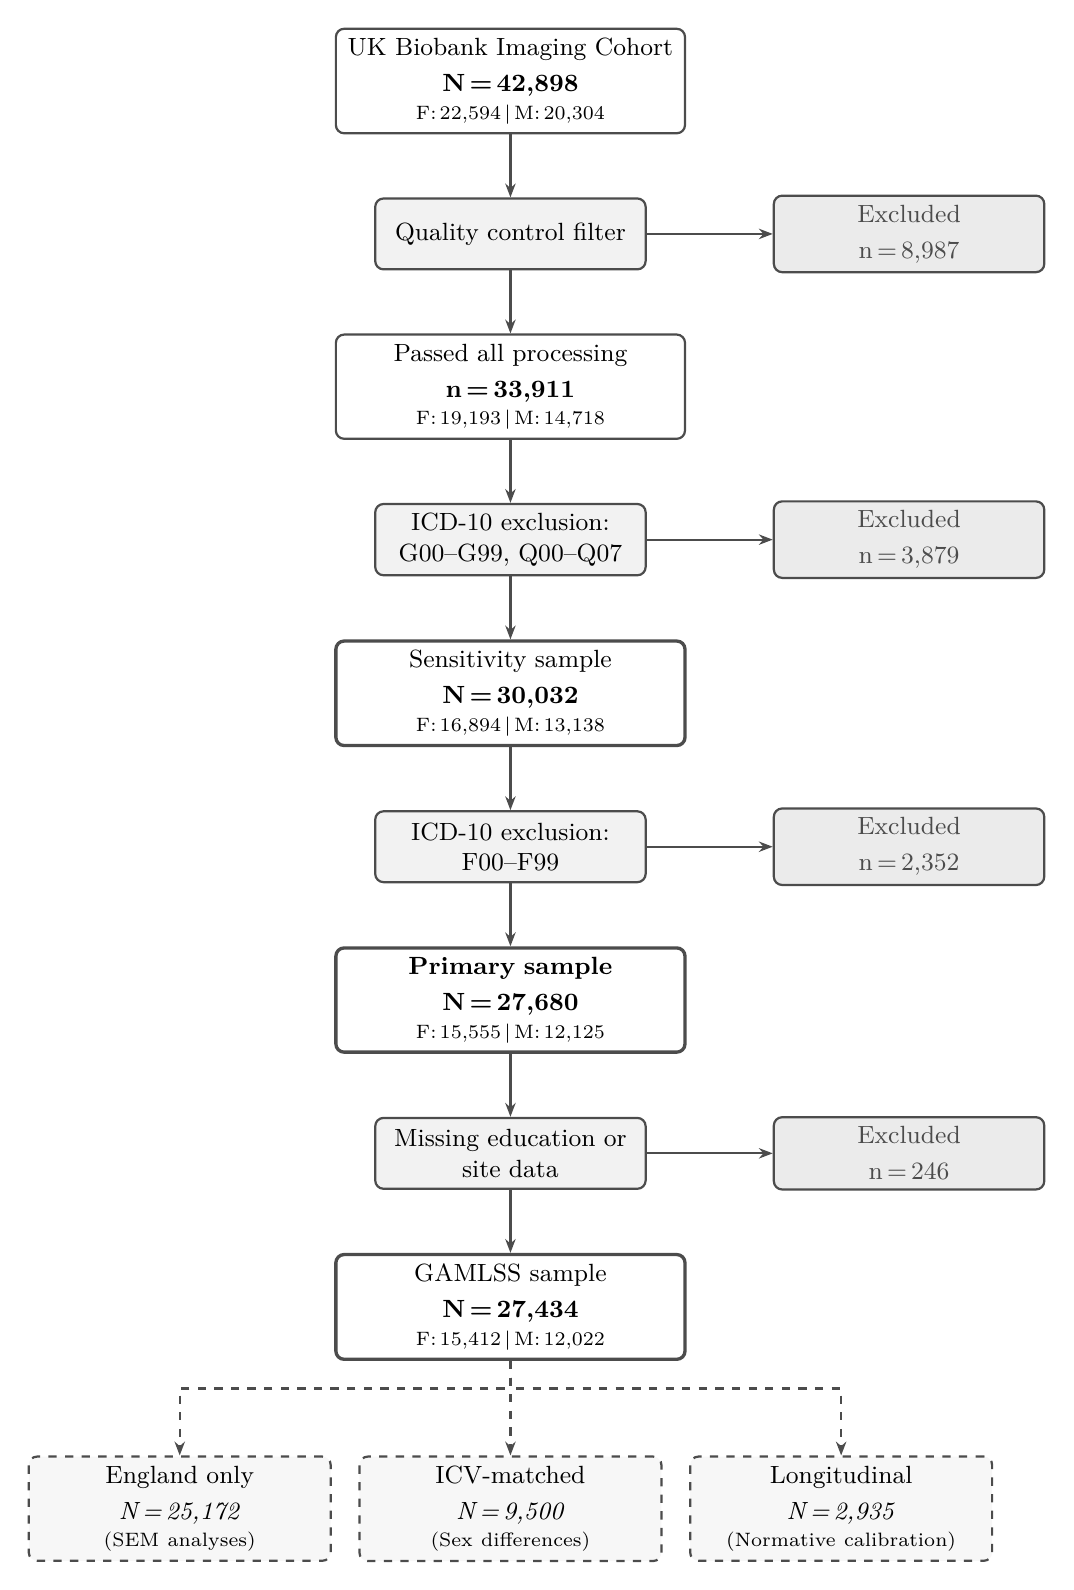
\begin{tikzpicture}[
  node distance=0.8cm and 1.6cm,
  every node/.style={font=\small},
  process/.style={rectangle, draw=black!70, thick, text width=4.2cm,
                  minimum height=0.9cm, align=center, rounded corners=3pt},
  decision/.style={rectangle, draw=black!70, thick, text width=3.2cm,
                   minimum height=0.9cm, align=center, rounded corners=3pt,
                   fill=black!5},
  excluded/.style={rectangle, draw=black!70, thick, text width=3.2cm,
                   minimum height=0.9cm, align=center, rounded corners=3pt,
                   fill=black!8, text=black!70},
  sample/.style={rectangle, draw=black!70, very thick, text width=4.2cm,
                 minimum height=0.9cm, align=center, rounded corners=3pt},
  subsample/.style={rectangle, draw=black!70, thick, text width=3.6cm,
                    minimum height=0.9cm, align=center, rounded corners=3pt,
                    fill=black!3, dashed},
  arrow/.style={-{Stealth[length=5pt]}, thick, black!70}
]
  % Main flow (top to bottom). All counts are unique participants;
  % sex-stratified Ns from R/scripts/audit_sex_balance.R.
  \node[process] (initial)
    {UK Biobank Imaging Cohort\\[2pt]\textbf{N\,=\,42,898}\\[-1pt]{\scriptsize F:\,22,594\,|\,M:\,20,304}};

  \node[decision, below=of initial] (qc)
    {Quality control filter};

  \node[process, below=of qc] (passed)
    {Passed all processing\\[2pt]\textbf{n\,=\,33,911}\\[-1pt]{\scriptsize F:\,19,193\,|\,M:\,14,718}};

  \node[decision, below=of passed] (gq)
    {ICD-10 exclusion:\\G00--G99, Q00--Q07};

  \node[sample, below=of gq] (sensitivity)
    {Sensitivity sample\\[2pt]\textbf{N\,=\,30,032}\\[-1pt]{\scriptsize F:\,16,894\,|\,M:\,13,138}};

  \node[decision, below=of sensitivity] (f)
    {ICD-10 exclusion:\\F00--F99};

  \node[sample, below=of f] (primary)
    {\textbf{Primary sample}\\[2pt]\textbf{N\,=\,27,680}\\[-1pt]{\scriptsize F:\,15,555\,|\,M:\,12,125}};

  \node[decision, below=of primary] (edu)
    {Missing education or\\site data};

  \node[sample, below=of edu] (gamlss)
    {GAMLSS sample\\[2pt]\textbf{N\,=\,27,434}\\[-1pt]{\scriptsize F:\,15,412\,|\,M:\,12,022}};

  % Exclusion boxes (right side)
  \node[excluded, right=of qc] (exc1)
    {Excluded\\[2pt]n\,=\,8,987};

  \node[excluded, right=of gq] (exc2)
    {Excluded\\[2pt]n\,=\,3,879};

  \node[excluded, right=of f] (exc3)
    {Excluded\\[2pt]n\,=\,2,352};

  \node[excluded, right=of edu] (exc4)
    {Excluded\\[2pt]n\,=\,246};

  % Subsamples (below GAMLSS, three across)
  \node[subsample, below=1.2cm of gamlss, xshift=-4.2cm] (england)
    {England only\\[2pt]\textit{N\,=\,25,172}\\[-1pt]{\scriptsize(SEM analyses)}};

  \node[subsample, below=1.2cm of gamlss] (matched)
    {ICV-matched\\[2pt]\textit{N\,=\,9,500}\\[-1pt]{\scriptsize(Sex differences)}};

  \node[subsample, below=1.2cm of gamlss, xshift=4.2cm] (longitudinal)
    {Longitudinal\\[2pt]\textit{N\,=\,2,935}\\[-1pt]{\scriptsize(Normative calibration)}};

  % Arrows
  \draw[arrow] (initial) -- (qc);
  \draw[arrow] (qc) -- (passed);
  \draw[arrow] (qc) -- (exc1);
  \draw[arrow] (passed) -- (gq);
  \draw[arrow] (gq) -- (sensitivity);
  \draw[arrow] (gq) -- (exc2);
  \draw[arrow] (sensitivity) -- (f);
  \draw[arrow] (f) -- (primary);
  \draw[arrow] (f) -- (exc3);
  \draw[arrow] (primary) -- (edu);
  \draw[arrow] (edu) -- (gamlss);
  \draw[arrow] (edu) -- (exc4);
  \draw[arrow, dashed] (gamlss.south) -- ++(0,-0.35cm) -| (england.north);
  \draw[arrow, dashed] (gamlss.south) -- (matched.north);
  \draw[arrow, dashed] (gamlss.south) -- ++(0,-0.35cm) -| (longitudinal.north);
\end{tikzpicture}
\end{document}
